\sectionp{3p}{Offline labelling of SWR segments}
\label{sec:offline}

To quantify the performance of a sharp wave-ripple (SWR) detection algorithm, we need an evaluation or `test' recording, annotated with the segments of time when actual SWR events were present. This section describes how such annotations can be made, and how our data specifically was annotated.

SWR's are an empirical phenomenon of hippocampal area CA1, `defined' by what their voltage traces look like. In other words, there is no ground truth available to know when SWR's occur. Scientists looking to annotate their LFP recordings with SWR segments therefore have to rely either on judgement calls by human labellers, or on an automated, offline SWR detection algorithm. The former could be considered more subjective, and is definitely more labour intensive than the latter -- especially if multiple scientists are consulted to obtain a consensus labelling. Most studies use an automated, offline algorithm to detect SWR segments (see \cref{apx:SWR-detection-literature} for some examples).

`Offline' here means that SWR detection happens after the recording has been completed, and that there are thus no real-time constraints on the detection algorithm. This means that 1) there are no hard bounds on algorithm execution time, and 2) that the algorithm can use information `from the future': when deciding whether a recording sample $\z_t$ belongs to an SWR segment, it can use samples $\z_{t_f}$ in its decision that occured after $\z_t$ (i.e. $t_f > t$), instead of using only past samples $\z_{t_p}$ (where $t_p \leq t$).



\subsection{Overview of offline ripple detection}

The main steps of the offline SWR detection algorithm that most studies use -- such as the ones cited in \cref{apx:SWR-detection-literature}, and this thesis itself -- can be summarized as follows:
\begin{enumerate}
\item Use a single channel of input data; namely from an electrode in the pyramidal cell layer of CA1, where the ripple part of SWR's is most strongly present. (We will denote this voltage signal with $z_t$);
\item Band-pass filter the recording to retain only `ripple' frequencies. (We will denote the filter output as $o_t$);
\item Obtain the envelope of the band-pass filtered signal. (We will denote this envelope with $n_t$);
\item Calculate a `high' and a `low' threshold ($T\high$ and $T\low$) to apply to the envelope $n_t$, based on summary statistics of $n_t$ and two custom multipliers ($\alpha\high$ and $\alpha\low$);
\item Define ripple events as times when the envelope crosses the high threshold (i.e. $n_t > T\high$);
\item Define the start and end time of each such ripple as the closest times where the envelope falls back below the lower threshold (i.e. $n_t < T\low$).
\end{enumerate}

\Cref{fig:offline-steps} visualizes each step, as applied to a fragment of our dataset. Note that this procedure only detects ripples, and not sharp waves.\footnote{Although interestingly, the sharp wave part of sharp wave-ripples was discovered before the ripple part \cite[p. 1]{Buzsaki2015}.}

\begin{figure}
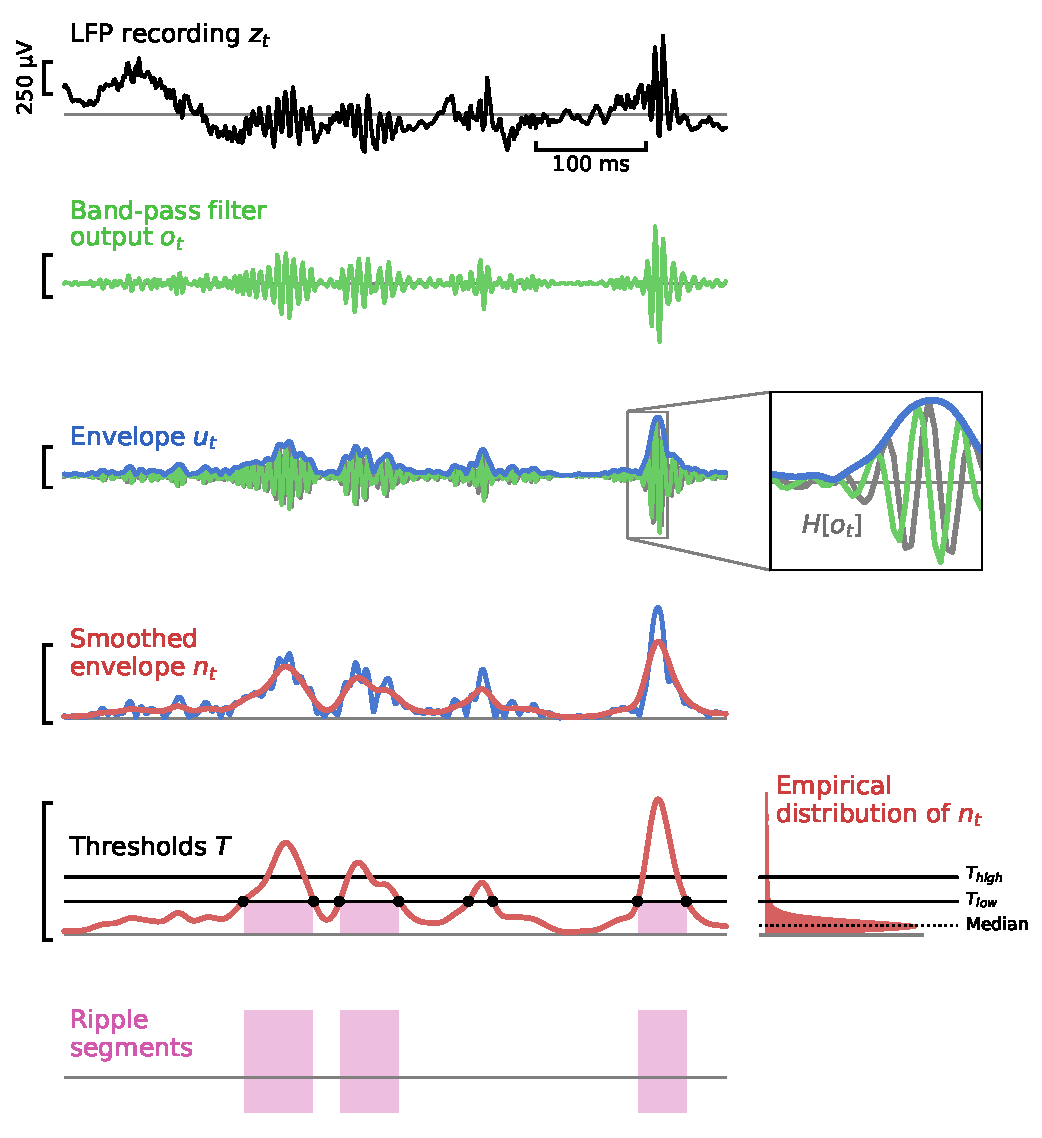
\includegraphics{figures/107_2--107_8}
\captionn{Steps for automated, offline SWR labelling}{See text for details. Each vertical scalebar indicates the same voltage range. $H[o_t]$ denotes the Hilbert transform of $o_t$. Note its phase lag of 90\si{\degree} with respect to $o_t$. In the second panel from the bottom, note the two threshold crossings of $T\low$ (marked with black dots) that did not result in a ripple segment, because the second threshold $T\high$ was not reached. The distribution of the envelope $n_t$ was estimated using the entire dataset (and not just the displayed fragment).}
\label{fig:offline-steps}
\end{figure}



\subsection{Validating parameter choices}
\label{sec:validating-parameter-choices}

Some of the above steps have free parameters (such as the ripple frequency band used for filtering, or the threshold multipliers $\alpha\high$ and $\alpha\low$). If not mentioned otherwise, our parameter choices were made as follows:

In a first pass of the offline detection algorithm, ripples were detected using a very broad-band filter and a low detection threshold. This ensured that all `true' SWR's were included in the detected events set (in addition to many spurious detections).

Next, five neuroscientists were independently asked to decide for each detected event whether it was an SWR event or not. This was done through a custom-made web app, an example screen of which is depicted in \cref{fig:labelface-UI}. Note that the labellers could factor multiple recording channels into their decision, including stratum radiatum channels displaying sharp wave activity. Only the events that were labelled as an SWR by at least three neuroscientists were retained.

Lastly, when setting the parameters of the final offline ripple detection algorithm, the algorithm's output was compared to the decisions made by the neuroscientists. The parameters were then adjusted until the output of the algorithm matched the neuroscientists' decisions reasonably well.

The following subsections describe the detection steps in more detail, and compare our choices of methods and parameters to those made in the literature.


\subsection{Band-pass filter design}

The wideband voltage signal $x_t$ was band-pass filtered between 100 and 200 Hz, using a linear, time-invariant filter with zero output lag.
% todo: mention downsampling

Many other studies use a higher left bound, of about 140--150 Hz (see \cref{tab:bands}). Using such a high bound however resulted in ripples that went undetected (even at low detection thresholds), although they were convicingly marked as SWR's by the neuroscientists.

The band-pass filter was designed using the windowed-sinc method, with a Kaiser window (using SciPy's \texttt{firwin} and \texttt{kaiserord} functions) \cite{Roelandts2016,Jones2018a}. The transition width was chosen to be 10\% of the bandwidth (i.e. 10 Hz), and the attenuation to be 40 dB, resulting in an FIR filter of order 150 (at a 1000 Hz sampling frequency).

The filter was applied bidirectionally, resulting in a zero-lag output, and a total attenuation of 80 dB. \Cref{fig:offline-steps} shows an example of the filter output in green.

We cannot compare our filter design method with the literature, as most studies do not mention such information.



\subsection{Envelope calculation}

Next, the instantaneous envelope $u_t$ of the filter output $o_t$ was calculated using its Hilbert transform\footnotemark{} $H[o_t]$:
%
\begin{equation}
\label{eq:Hilbert_envelope}
u_t = \sqrt{o_t^2 + H[o_t]^2},
\end{equation}

\footnotetext{To be precise, $H$ is a discrete approximation to the continuous Hilbert transform $\mathcal{H}$. There are multiple ways to make a discrete approximation to $\mathcal{H}$ \cite{Oppenheim2009}. Most of them make use of the discrete Fourier transform, which makes computing $H$ an efficient operation. We used SciPy's \texttt{hilbert} function (which, confusingly, does not return the Hilbert transform of its input, but rather its analytical signal), and zero-padded the input signal to the nearest power of 2 or 3 to benefit from the speedup brought by the fast Fourier transform algorithm.}

The Hilbert transform delays each frequency component of a signal by 90\si{\degree} \cite{Lyons2010} (see the gray signal in \cref{fig:offline-steps}). This means that the envelope of a narrowband signal such as $o_t$ can be easily obtained as the magnitude of the so called `analytic signal' $o_t + j H[o_t]$, as in \cref{eq:Hilbert_envelope}.\footnotemark{}

\footnotetext{To see why, consider a local approximation of the narrowband signal $o_t$ by a sinusoid $a \cos{\omega t}$. Its Hilbert transform is then $a \sin{\omega t}$. From \cref{eq:Hilbert_envelope}, the envelope $u_t$ will be locally approximated by the magnitude of the original signal: $u_t = \sqrt{(a \cos{\omega t})^2 + (a \sin{\omega t})^2} = \abs{a}$.}

After calculating $u_t$, a final, smoothed envelope $n_t$ was obtained by convolving $u_t$ with a Gaussian kernel ($\sigma$ = 7.5 ms, support radius of $4 \sigma$). Compare the blue ($u_t$) and the red signal ($n_t$) in \cref{fig:offline-steps}.

Other studies (such as \cite{Nadasdy1999} and \cite{Csicsvari2000}) use a ``root-mean-square'' approach to calculate the envelope of the filter output $o_t$. In these studies, presumably, the squared signal $o_t^2$ is smoothed using some kernel (of unspecified type and bandwidth) to obtain the ``mean-square'' signal of which the square root is taken.



\subsection{Threshold calculation}

The two detection thresholds were calculated as follows:
\begin{align}
\label{eq:thresholds-symbolic}
T\high &= \alpha\high \times \median{n_t} \\
T\low  &= \alpha\low  \times \median{n_t}
\end{align}
%
where $\median{n_t}$ denotes the median of the smoothed envelope $n_t$. As per the procedure described in ``\nameref{sec:validating-parameter-choices}'', we set $\alpha\high = 6.2$ and $\alpha\low = 3.6$. At a median envelope magnitude $\median{n_t} = \SI{17.0}{\micro\volt}$, this results in thresholds $T\high = \SI{105.4}{\micro\volt}$ and $T\low = \SI{61.2}{\micro\volt}$.

Most studies calculate thresholds as follows: $T\high = \mean{n_t} + \beta\high \times \std(n_t)$. Here $\mean{n_t}$ denotes the mean of the envelope, $\std(n_t)$ denotes its standard deviation, and $\beta\high$ is a custom multiplier analogous to $\alpha\high$. For the non-negative, assymetric distributions of envelope signals, using both a measure of center and a measure of spread to define thresholds seems unnecessary (see the distribution of $n_t$ in \cref{fig:offline-steps}), which is why we chose to use only one measure (namely the median).
% One advantage of the median over the mean, is that the former is far less sensitive to outliers of than the latter. Our dataset did not seem to include any outliers, such as erroneous samples with improbably high magnitude, however.

The detection multiplier $\beta\high$ varies wildly between studies: from 1, over 3, 4, and 5, up until 7 (\cite{Csicsvari2000,Dutta2018,Behrens2005,Sadowski2016,Nadasdy1999}, respectively).\footnotemark{} It is clear that such different thresholds will give very different sensitivity-precision trade-offs for SWR detection (the lower thresholds yielding more false positive detections, and the higher thresholds yielding more missed true SWR events).

\footnotetext{Threshold multipliers cannot be compared precisely: a different background `noise' level or ripple incidence rate will result in different $\mean{n_t}$ and $\std(n_t)$ values. This means that $\beta\high$ needs to change to maintain an equal threshold $T\high$; which is necessary when the ripples to be detected have not changed their magnitude.}

To compare our thresholds to those in the literature, we calculate the $\beta$ multipliers corresponding to our chosen $\alpha$ values. Given that our dataset has a mean envelope magnitude of 22.3 \uV{} and a standard deviation of 22.9 \uV{}, we find $\beta\high = 3.63$ and $\beta\low = 1.70$. These values fall near the center of those reported in the literature (see \cref{apx:SWR-detection-literature}).
% todo: calculate ripple magnitude and background magnitude



\subsection{Segment post-processing}

Finally, two add-hoc rules were applied to the automatically detected ripple segments. First, segments with only a small gap between them (of less than 10 ms) were joined together. Then, segments of too short a duration (less than 25 ms) were eliminated.

This step is rarely done in other studies. An exception is e.g. \cite{Dutta2018}, were segments shorter than 15 ms were eliminated.



% todo: standardized data
